\documentclass[conference]{IEEEtran}
% Relatorio incremental do mestrado (formato IEEE conference).
% Compilar com pdfLaTeX (Overleaf: Menu > Compiler > pdfLaTeX).

\usepackage[utf8]{inputenc}
\usepackage[T1]{fontenc}
\usepackage[brazil]{babel}
\usepackage{cite}
\usepackage{amsmath,amssymb,amsfonts}
\usepackage{graphicx}
\usepackage{booktabs}
\usepackage{multirow}
\usepackage{textcomp}
\usepackage{xcolor}
\usepackage{url}

% Marcador para valores ainda nao obtidos (treinos em execucao)
\newcommand{\pend}{\textcolor{gray}{--}}
% Marcador para trechos a revisar/completar pelo autor
\newcommand{\todo}[1]{\textcolor{red}{[#1]}}

\begin{document}

\title{Replicação do \textit{Reflective Gaussian Splatting} e Propostas para a Modelagem de Visibilidade em Superfícies Reflexivas}

\author{\IEEEauthorblockN{João Pedro Maciel Pimenta}
\IEEEauthorblockA{\textit{Centro de Informática} \\
\textit{Universidade Federal de Pernambuco}\\
Recife, Brasil \\
jpmp3@cin.ufpe.br}
\and
\IEEEauthorblockN{Francisco Paulo Magalhães Simões}
\IEEEauthorblockA{\textit{Centro de Informática} \\
\textit{Universidade Federal de Pernambuco}\\
Recife, Brasil \\
fpms@cin.ufpe.br}
}

\maketitle

\begin{abstract}
A reconstrução de superfícies reflexivas continua sendo um ponto fraco dos métodos de síntese de novas vistas baseados em Gaussian Splatting, pois a aparência dependente da direção de observação é aprendida sem um modelo físico explícito da luz refletida. O Reflective Gaussian Splatting (Ref-Gaussian) aborda o problema com renderização diferida fisicamente baseada sobre Gaussianas 2D e com um termo de inter-reflexão calculado por ray tracing sobre uma malha extraída periodicamente da cena. Este relatório descreve o método, identifica suas limitações quanto à aproximação de visibilidade e ao custo da extração de malha, e propõe duas linhas de investigação para a dissertação. Como primeiro passo experimental, o código oficial foi portado e executado em uma GPU de notebook sob Windows, e o baseline foi replicado no conjunto Shiny Blender Synthetic. Nas duas cenas concluídas, os resultados ficam próximos aos do artigo original: na toaster, PSNR de 27,51 dB, SSIM de 0,948 e LPIPS de 0,074, contra 28,05 dB, 0,948 e 0,074; na ball, 36,07 dB, 0,985 e 0,089, contra 37,01 dB, 0,981 e 0,098. A comparação entre uma cena côncava, com inter-reflexões, e uma convexa, sem elas, mostra que os erros e o ruído nos materiais se concentram onde a visibilidade importa, o que motiva as propostas.
\end{abstract}

\begin{IEEEkeywords}
Gaussian Splatting, superfícies reflexivas, renderização fisicamente baseada, inter-reflexão, síntese de novas vistas.
\end{IEEEkeywords}

% =====================================================================
\section{Introdução}

O 3D Gaussian Splatting (3DGS)~\cite{kerbl2023} representa uma cena como um conjunto de Gaussianas anisotrópicas rasterizadas de forma diferenciável, alcançando qualidade comparável à dos campos de radiância neurais com renderização em tempo real. Sua aparência dependente de vista, porém, é modelada por harmônicos esféricos de baixa ordem, o que é insuficiente para superfícies especulares: reflexos nítidos são aprendidos como geometria falsa ``atrás'' do objeto e as normais resultantes ficam incorretas.

\begin{table}[t]
\centering
\caption{PSNR no Shiny Blender reportado por Yao et al.~\cite{yao2025refgaussian} para métodos anteriores, como contexto para o baseline.}
\label{tab:sota}
\setlength{\tabcolsep}{3pt}
\begin{tabular}{lccccccc}
\toprule
Método & Ball & Car & Coffee & Helmet & Teapot & Toaster \\
\midrule
3DGS~\cite{kerbl2023}                    & 27,65 & 27,26 & 32,30 & 28,22 & 45,71 & 20,99 \\
2DGS~\cite{huang2024_2dgs}               & 25,97 & 26,38 & 32,31 & 27,42 & 44,97 & 20,42 \\
Ref-NeRF~\cite{verbin2022refnerf}        & 33,16 & 30,44 & 33,99 & 29,94 & 45,12 & 26,12 \\
GShader~\cite{jiang2024gaussianshader}   & 30,99 & 27,96 & 32,39 & 28,32 & 45,86 & 26,28 \\
3DGS-DR~\cite{ye2024dr}                  & 33,43 & 30,48 & 34,53 & 31,44 & 47,04 & 26,76 \\
Ref-Gaussian~\cite{yao2025refgaussian}   & \textbf{37,01} & \textbf{31,04} & \textbf{34,63} & \textbf{32,32} & \textbf{47,16} & \textbf{28,05} \\
\bottomrule
\end{tabular}
\end{table}

Trabalhos recentes incorporam modelos de sombreamento ao 3DGS. O GaussianShader~\cite{jiang2024gaussianshader} associa a cada Gaussiana uma função de sombreamento simplificada; o 3DGS-DR~\cite{ye2024dr} adia o cálculo da reflexão para o espaço da imagem; e o Ref-Gaussian~\cite{yao2025refgaussian}, adotado aqui como \textit{baseline}, combina Gaussianas 2D~\cite{huang2024_2dgs}, renderização diferida fisicamente baseada e um termo de inter-reflexão. O Ref-Gaussian supera os métodos anteriores no Shiny Blender~\cite{verbin2022refnerf} em todas as cenas (Tabela~\ref{tab:sota}).

Este relatório tem dois objetivos: (i) descrever o método base e as linhas de investigação propostas para a dissertação (Seção~\ref{sec:metodo}); e (ii) replicar os resultados do baseline em hardware de consumo, condição necessária antes de propor modificações (Seções~\ref{sec:exp} e~\ref{sec:resultados}).

% =====================================================================
\section{Solução Proposta}\label{sec:metodo}

\subsection{Método base: Reflective Gaussian Splatting}

A Fig.~\ref{fig:pipeline} resume o pipeline do Ref-Gaussian. Seus componentes são descritos a seguir.

\begin{figure*}[t]
\centering
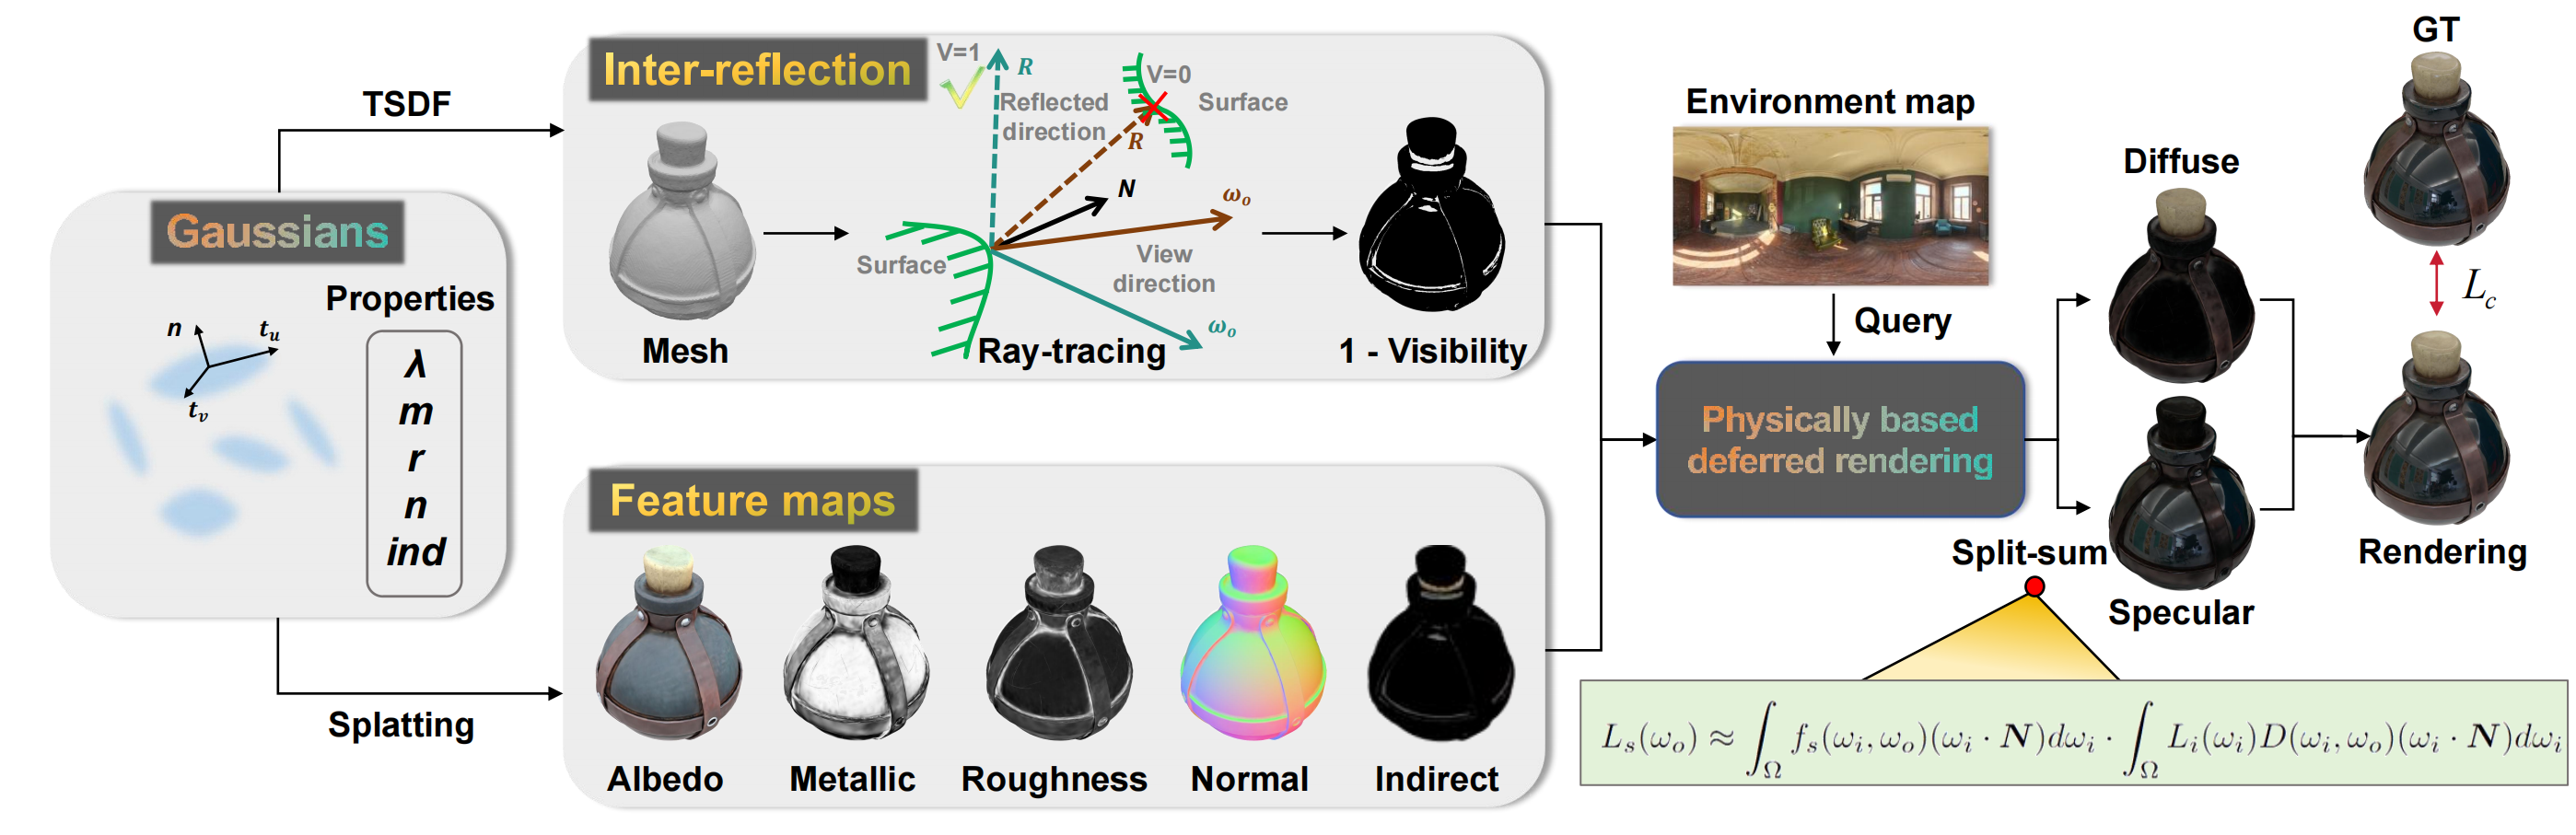
\includegraphics[width=0.92\textwidth]{figs/pipeline_refgaussian.png}
\caption{Pipeline do Ref-Gaussian: Gaussianas 2D com atributos de material são rasterizadas em mapas por pixel (renderização diferida); o sombreamento combina iluminação direta de um mapa de ambiente com inter-reflexão fundamentada nas próprias Gaussianas. Fonte: Yao et al.~\cite{yao2025refgaussian}.}
\label{fig:pipeline}
\end{figure*}

\begin{table*}[t]
\centering
\caption{Replicação do Ref-Gaussian no Shiny Blender Synthetic: valores reportados no artigo~\cite{yao2025refgaussian} e obtidos neste trabalho (RTX 4050 Laptop); $\Delta$ é a diferença de PSNR da replicação em relação ao artigo. ``--'' indica treino em andamento.}
\label{tab:replicacao}
\begin{tabular}{llccccccc}
\toprule
Métrica & Origem & Ball & Car & Coffee & Helmet & Teapot & Toaster & Média \\
\midrule
% Linhas geradas por atualizar_resultados.py a partir de ref-gaussian/output/<cena>/metric.txt
\csname @@input\endcsname tab_replicacao.tex
\bottomrule
\end{tabular}
\end{table*}

\begin{figure*}[t]
\centering
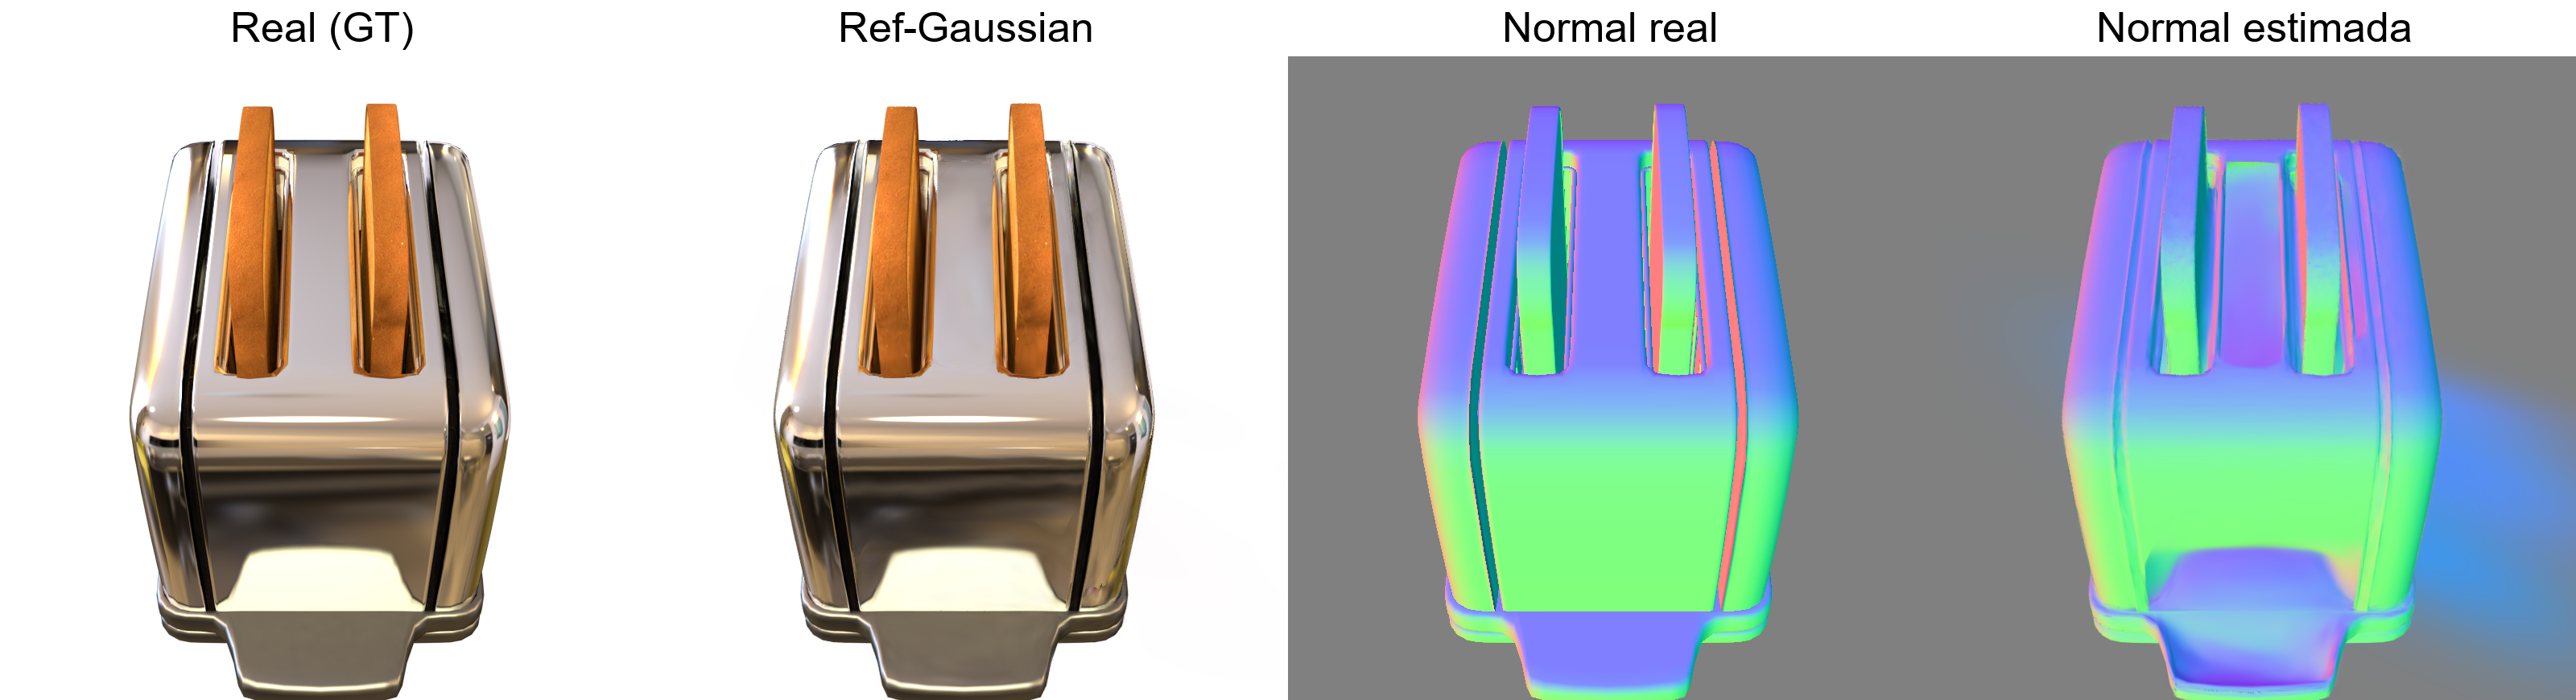
\includegraphics[width=\textwidth]{figs/toaster_qualitativo.png}
\caption{Resultado qualitativo na cena \textit{toaster} (vista de teste 0) após 50.000 iterações. Da esquerda para a direita: imagem real, renderização do Ref-Gaussian, normal real e normal estimada.}
\label{fig:toaster}
\end{figure*}

\textbf{Representação.} A cena é composta por \textit{surfels} Gaussianos 2D~\cite{huang2024_2dgs}, discos orientados definidos por centro, dois vetores tangentes, escalas e opacidade. A normal de cada primitiva é o vetor perpendicular ao seu plano, o que fornece geometria de superfície mais precisa que a das Gaussianas 3D. Cada primitiva carrega ainda os atributos de material do modelo Disney/PBR: albedo $\mathbf{a}$, metalicidade $m$ e rugosidade $r$.

\textbf{Renderização diferida.} Em vez de sombrear cada Gaussiana e depois combinar as cores, os atributos ($\mathbf{a}$, $m$, $r$, normal $\mathbf{n}$ e profundidade) são primeiro combinados por \textit{alpha blending} em mapas por pixel. O sombreamento é então avaliado uma única vez por pixel, o que gera reflexos mais nítidos e consistentes. A radiância de saída na direção $\boldsymbol{\omega}_o$ é dividida em um termo difuso e um especular:
\begin{equation}
L(\boldsymbol{\omega}_o) = L_d + L_s, \quad L_d = (1-m)\,\mathbf{a}\, \frac{1}{\pi}\!\int_{\Omega} L_i(\boldsymbol{\omega}_i)\,(\boldsymbol{\omega}_i\cdot\mathbf{n})\,d\boldsymbol{\omega}_i .
\end{equation}
O termo especular usa a aproximação \textit{split-sum}~\cite{karis2013}:
\begin{equation}
L_s \approx \big(\mathbf{F}_0\,A(\mathbf{n}\cdot\boldsymbol{\omega}_o, r) + B(\mathbf{n}\cdot\boldsymbol{\omega}_o, r)\big)\; \tilde{L}(\boldsymbol{\omega}_r, r),
\end{equation}
com $\mathbf{F}_0 = 0{,}04(1-m) + m\,\mathbf{a}$, termos $A$ e $B$ pré-integrados da BRDF em uma tabela, e $\tilde{L}$ a iluminação pré-filtrada amostrada na direção de reflexão $\boldsymbol{\omega}_r$ em um mapa de ambiente cúbico treinável com níveis de mipmap indexados pela rugosidade.

\textbf{Inter-reflexão fundamentada em Gaussianas.} O mapa de ambiente representa apenas luz vinda do infinito; reflexos de uma parte do objeto sobre outra exigem um termo indireto. O Ref-Gaussian separa a componente especular em
\begin{equation}
L_s = V\,L_s^{\text{dir}} + (1-V)\,L_s^{\text{ind}}, \qquad V\in\{0,1\},
\label{eq:vis}
\end{equation}
em que a visibilidade $V$ é obtida lançando um único raio na direção de reflexão $\boldsymbol{\omega}_r$ contra uma malha extraída das Gaussianas por fusão TSDF. A radiância indireta $L_s^{\text{ind}}$ é obtida da própria representação Gaussiana da cena. A malha é reextraída periodicamente durante o treino.

\textbf{Propagação de normais sensível ao material.} Para corrigir normais em regiões altamente especulares, as Gaussianas com $m \geq 0{,}02$ e $r \leq 0{,}1$ têm suas escalas periodicamente ampliadas, propagando normais corretas para as vizinhas.

\textbf{Treinamento em estágios.} O treino começa com sombreamento por Gaussiana, que estabiliza a geometria, e depois passa à renderização diferida. A função de perda é
\begin{equation}
\mathcal{L} = \mathcal{L}_c + \lambda_n \mathcal{L}_n + \lambda_s \mathcal{L}_{\text{smooth}},
\end{equation}
com $\mathcal{L}_c$ a perda fotométrica, $\mathcal{L}_n$ a consistência entre normais renderizadas e derivadas da profundidade~\cite{huang2024_2dgs} e $\mathcal{L}_{\text{smooth}}$ uma suavização de normais. O artigo usa $\lambda_n=0{,}05$ e $\lambda_s=1{,}0$.

\subsection{Limitações identificadas}

\begin{enumerate}
\item \textbf{Visibilidade pontual.} A Eq.~\eqref{eq:vis} testa a oclusão apenas na direção de reflexão especular perfeita e usa esse único teste para todo o lóbulo especular. Os próprios autores apontam que isso introduz ruído na estimativa de materiais. O erro tende a crescer com a rugosidade, quando o lóbulo se alarga.
\item \textbf{Dependência de malha extraída.} O ray tracing exige reconstruir uma malha por TSDF a cada poucos milhares de iterações e reconstruir a estrutura de aceleração (BVH). Isso adiciona custo, cria uma segunda representação geométrica que pode divergir das Gaussianas e torna a visibilidade não diferenciável em relação a elas.
\item \textbf{Escopo.} O método é desenhado para cenas estáticas e predominantemente especulares; os autores reconhecem desempenho inferior em cenas não especulares.
\end{enumerate}

\subsection{Linhas de investigação propostas}

As propostas a seguir são hipóteses de trabalho para a dissertação e serão avaliadas contra o baseline replicado neste relatório.

\textbf{P1 -- Visibilidade sobre o lóbulo especular.} Substituir o teste binário único por uma estimativa da visibilidade média sobre o lóbulo da BRDF:
\begin{equation}
\bar{V} \approx \frac{1}{K}\sum_{k=1}^{K} V(\boldsymbol{\omega}_k), \quad \boldsymbol{\omega}_k \sim D_{\text{GGX}}(\,\cdot\,;\boldsymbol{\omega}_r, r),
\end{equation}
com poucas direções $\boldsymbol{\omega}_k$ obtidas por amostragem por importância da distribuição GGX, de forma estratificada e com $K$ adaptativo à rugosidade ($K=1$ recupera o baseline em superfícies espelhadas). Para manter o custo baixo, serão avaliadas reutilização temporal das amostras entre iterações e aproximações por cone. A avaliação usará PSNR/SSIM/LPIPS, o erro de albedo e rugosidade nas cenas sintéticas com material conhecido, e uma ablação de $K$ contra tempo de treino.

\textbf{P2 -- Visibilidade direta a partir das primitivas.} Eliminar a extração de malha calculando a oclusão diretamente sobre as Gaussianas, acumulando a transmitância ao longo do raio refletido com uma estrutura de aceleração sobre envelopes das primitivas, na linha do ray tracing de Gaussianas~\cite{moenne2024_3dgrt}. Além de remover o custo do TSDF, essa formulação permite uma visibilidade contínua e potencialmente diferenciável em relação à geometria. As métricas são as mesmas de P1, mais o tempo total de treino e o consumo de memória.

\textbf{P3 -- Extensão dinâmica (trabalho futuro).} Estender a representação por Gaussianas 2D a objetos reflexivos em movimento, tratando a coerência temporal dos reflexos. Esta linha depende dos resultados de P1/P2 e fica como perspectiva.

% =====================================================================
\section{Experimentos}\label{sec:exp}

O objetivo desta etapa é replicar o baseline com o código oficial antes de qualquer modificação.

\subsection{Ambiente e reprodutibilidade}

Os experimentos usam o código oficial do Ref-Gaussian (commit \texttt{af7691a}, mar.~2025) em um notebook com GPU NVIDIA GeForce RTX 4050 Laptop (6~GB), Windows~11, CUDA~11.8, PyTorch~2.0.0 e Python~3.8. O código foi desenvolvido para Linux, e as extensões CUDA (rasterizador de \textit{surfels}, \textit{simple-knn}, codificador de cubemap e o ray tracer baseado em BVH) precisaram de ajustes para compilar com o MSVC~14.44 (Visual Studio~2022), mais recente que o oficialmente suportado pelo CUDA~11.8. Os principais ajustes foram: permitir o compilador não suportado; incluir explicitamente cabeçalhos que o GCC inclui de forma transitiva; ativar o modo de conformidade do MSVC (\texttt{/permissive-}, \texttt{/Zc:\_\_cplusplus}), necessário para compilar a biblioteca Eigen junto com o nvcc; e impedir a inclusão do pybind11 nos arquivos CUDA. Nenhum desses ajustes altera o código-fonte do método; todos foram feitos por meio de flags de compilação, registradas em scripts no repositório do projeto.

\subsection{Conjunto de dados}

Nesta etapa usa-se o Shiny Blender Synthetic~\cite{verbin2022refnerf}, com seis objetos sintéticos de materiais altamente especulares (\textit{ball}, \textit{car}, \textit{coffee}, \textit{helmet}, \textit{teapot} e \textit{toaster}). Cada cena tem 100 vistas de treino e 200 de teste, em resolução $800\times800$ e fundo branco. Os conjuntos Glossy Synthetic~\cite{liu2023nero} e Shiny Blender Real serão usados nas próximas etapas.

\subsection{Protocolo}

O treino segue os argumentos do script \texttt{train.sh} do repositório oficial, com a configuração padrão do código: 50.000 iterações, sombreamento por Gaussiana até a iteração 18.000, inter-reflexão a partir da iteração 20.000, extração de malha (resolução 512) a cada 2.000 iterações e densificação até a iteração 25.000. As cenas \textit{helmet} e \textit{ball} usam $\lambda_s=1{,}0$, como no script oficial. Esse cronograma difere do descrito no artigo (18.000 iterações iniciais mais 40.000 com renderização diferida, extração a cada 3.000 passos); optou-se pela configuração publicada no código.

As métricas são as do artigo, calculadas pelo script de avaliação oficial sobre as 200 vistas de teste: PSNR, SSIM e LPIPS (VGG). Reportam-se também a taxa de renderização (FPS) e o tempo de treino.

% =====================================================================
\section{Resultados e Discussão}\label{sec:resultados}

\textbf{Métricas.} A Tabela~\ref{tab:replicacao} compara os resultados obtidos com os do artigo. Na cena \textit{toaster}, a mais difícil do conjunto para todos os métodos (Tabela~\ref{tab:sota}), o SSIM e o LPIPS replicados coincidem com os reportados até a terceira casa decimal, e o PSNR fica 0,54~dB abaixo. A diferença é pequena diante da variação esperada entre execuções de métodos com treino estocástico, e há fatores conhecidos que podem explicá-la: GPU, versão do compilador e não determinismo das operações atômicas na rasterização. Há também a diferença de cronograma de treino descrita na Seção~\ref{sec:exp}. Mesmo 0,54~dB abaixo, o resultado supera em 0,75~dB o melhor método anterior nessa cena (3DGS-DR). Na cena \textit{ball}, o PSNR replicado é de 36,07~dB, 0,94~dB abaixo do artigo, enquanto o SSIM (0,985 contra 0,981) e o LPIPS (0,089 contra 0,098) ficam \emph{melhores} que os reportados. A qualidade estrutural e perceptual é, portanto, reproduzida integralmente, e o déficit se limita a um erro fotométrico pequeno e difuso. Ainda assim, o resultado está 2,64~dB acima do melhor método anterior nessa cena (3DGS-DR, 33,43~dB). As quatro cenas restantes (\textit{car}, \textit{coffee}, \textit{helmet} e \textit{teapot}) estão em treino e completarão a tabela na próxima entrega.

\begin{table}[t]
\centering
\caption{Custo na RTX 4050 Laptop: tempo de treino (50.000 iterações) e taxa de renderização na avaliação.}
\label{tab:custo}
\begin{tabular}{lcc}
\toprule
Cena & Tempo de treino & FPS \\
\midrule
% Linhas geradas por atualizar_resultados.py
\csname @@input\endcsname tab_custo.tex
\bottomrule
\end{tabular}
\end{table}

\begin{figure}[t]
\centering
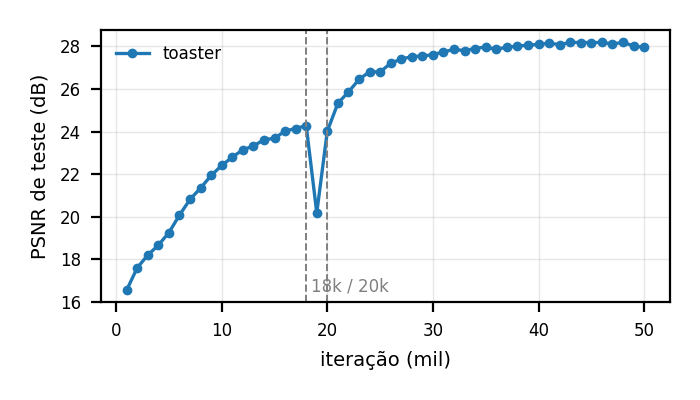
\includegraphics[width=\columnwidth]{figs/curvas_psnr.png}
\caption{PSNR nas vistas de teste ao longo do treino da cena \textit{toaster} (a \textit{ball} foi treinada sem registro do log). As linhas tracejadas marcam o fim do sombreamento por Gaussiana (18 mil iterações) e o início da inter-reflexão (20 mil).}
\label{fig:curvas}
\end{figure}

\textbf{Dinâmica do treino.} A Fig.~\ref{fig:curvas} mostra a evolução do PSNR de teste, medido pelo próprio script de treino a cada mil iterações. Na cena \textit{toaster}, o estágio de sombreamento por Gaussiana leva o PSNR a cerca de 24,3~dB na iteração 18 mil. A troca para a renderização diferida derruba o valor temporariamente para 20,2~dB, já que os mapas de material passam a ser combinados antes do sombreamento, mas ele se recupera em menos de 2 mil iterações. A partir da inter-reflexão (20 mil), o PSNR sobe para cerca de 28,2~dB em torno de 43 mil iterações; esse ganho de quase 4~dB após a etapa inicial indica que a renderização diferida e o termo indireto respondem por boa parte da qualidade final. Nas últimas milhares de iterações há uma leve queda (de 28,19 para 27,96~dB). Além disso, o script de avaliação mede 27,51~dB sobre as mesmas 200 vistas, 0,45~dB abaixo da medição feita durante o treino; a origem dessa diferença entre os dois scripts ainda será investigada. Esses dois pontos indicam que parte da distância para o artigo pode estar no protocolo de medição e na escolha do checkpoint, e não no método.

\textbf{Custo computacional.} A Tabela~\ref{tab:custo} resume o custo por cena. O treino completo da cena \textit{toaster} levou cerca de 1h46min, e a renderização na avaliação atingiu 38,9~FPS. O artigo reporta 0,58~h de treino em média e 122~FPS em uma NVIDIA A6000. A diferença é coerente com a distância de capacidade entre uma GPU de notebook de 6~GB e uma GPU de estação de trabalho de 48~GB. Ainda assim, mostra que o baseline pode ser treinado integralmente em hardware de consumo, o que viabiliza os experimentos da dissertação. A \textit{ball} treinou mais rápido (1h25min), coerente com seu modelo menor (38 mil Gaussianas e malha de 76 mil vértices, contra 83 mil e 126 mil na \textit{toaster}). Seu FPS na avaliação (10,6), porém, foi menor apesar do modelo menor, o que indica interferência do estado da máquina no momento da medição, como modo de energia ou outros processos na GPU. As medições de FPS serão repetidas em condições controladas antes de qualquer comparação de desempenho.

\textbf{Análise qualitativa.} Na Fig.~\ref{fig:toaster}, a renderização reproduz os reflexos especulares do corpo metálico, incluindo os reflexos das fatias de pão sobre a carcaça, uma situação de inter-reflexão. O mapa de normais estimado, por outro lado, é mais suave que o real: os frisos verticais estreitos nas laterais praticamente desaparecem, e surgem artefatos de baixa opacidade no fundo, fora do objeto. Esse descompasso entre aparência correta e geometria aproximada é relevante para as propostas da Seção~\ref{sec:metodo}. Como a visibilidade do baseline é calculada sobre uma malha derivada dessa geometria, erros finos de normal e de superfície se propagam para o termo de inter-reflexão. Esse efeito motiva tanto a amostragem do lóbulo (P1) quanto a visibilidade calculada diretamente sobre as primitivas (P2).

\begin{figure}[t]
\centering
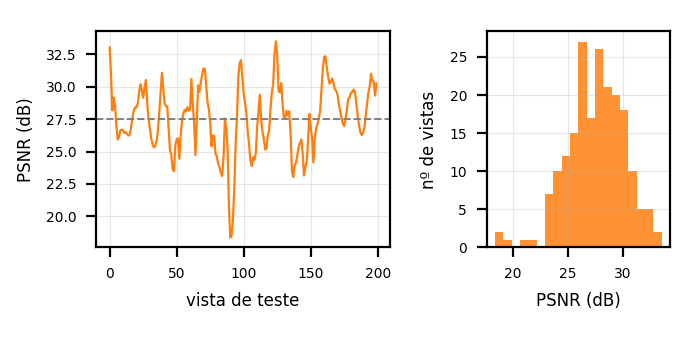
\includegraphics[width=\columnwidth]{figs/toaster_psnr_vistas.png}
\caption{PSNR por vista de teste na cena \textit{toaster}: valor de cada uma das 200 vistas (esquerda, linha tracejada na média) e histograma (direita).}
\label{fig:vistas}
\end{figure}

\begin{figure*}[t]
\centering
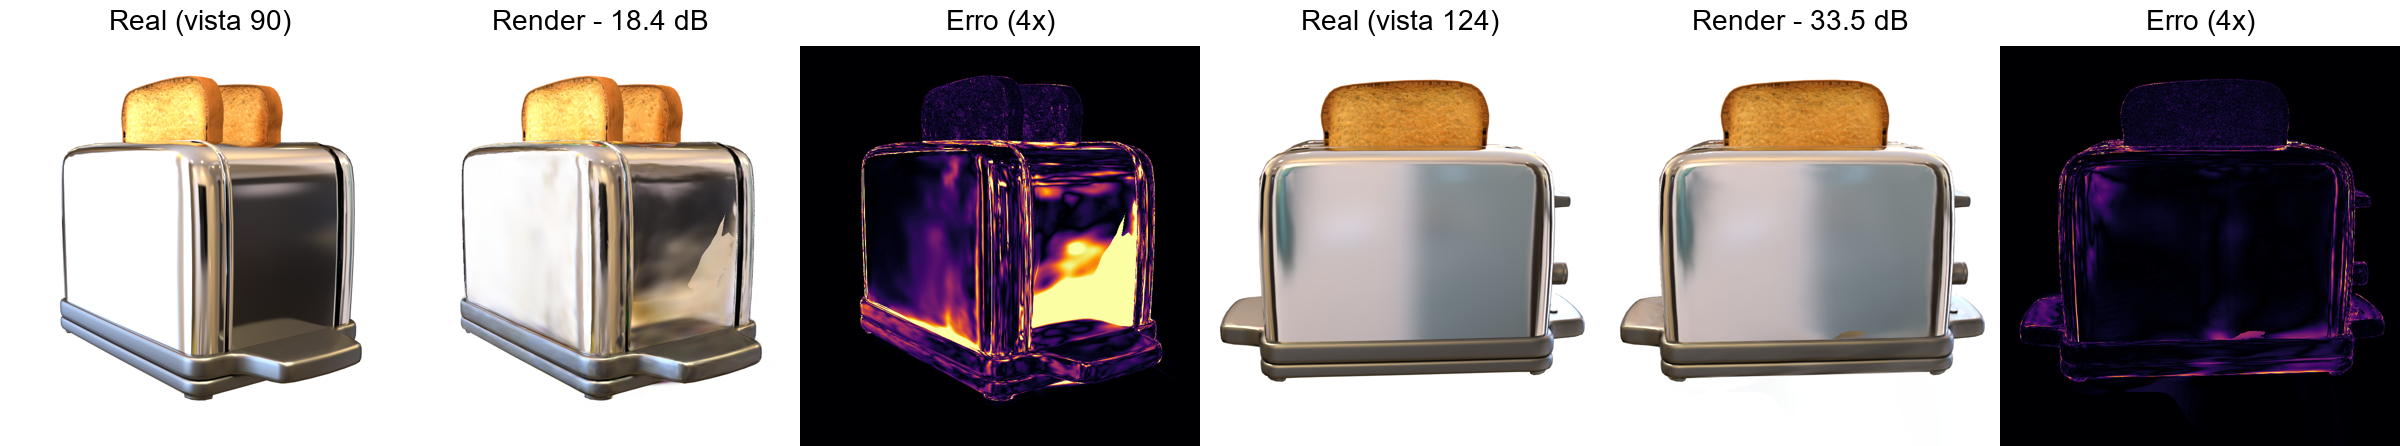
\includegraphics[width=\textwidth]{figs/toaster_extremos.png}
\caption{Pior (vista 90, 18,4~dB) e melhor (vista 124, 33,5~dB) vistas de teste da cena \textit{toaster}, com o erro absoluto amplificado 4 vezes. Na pior vista, a lateral espelhada, que na imagem real reflete uma região escura, é renderizada clara.}
\label{fig:extremos}
\end{figure*}

\begin{figure*}[t]
\centering
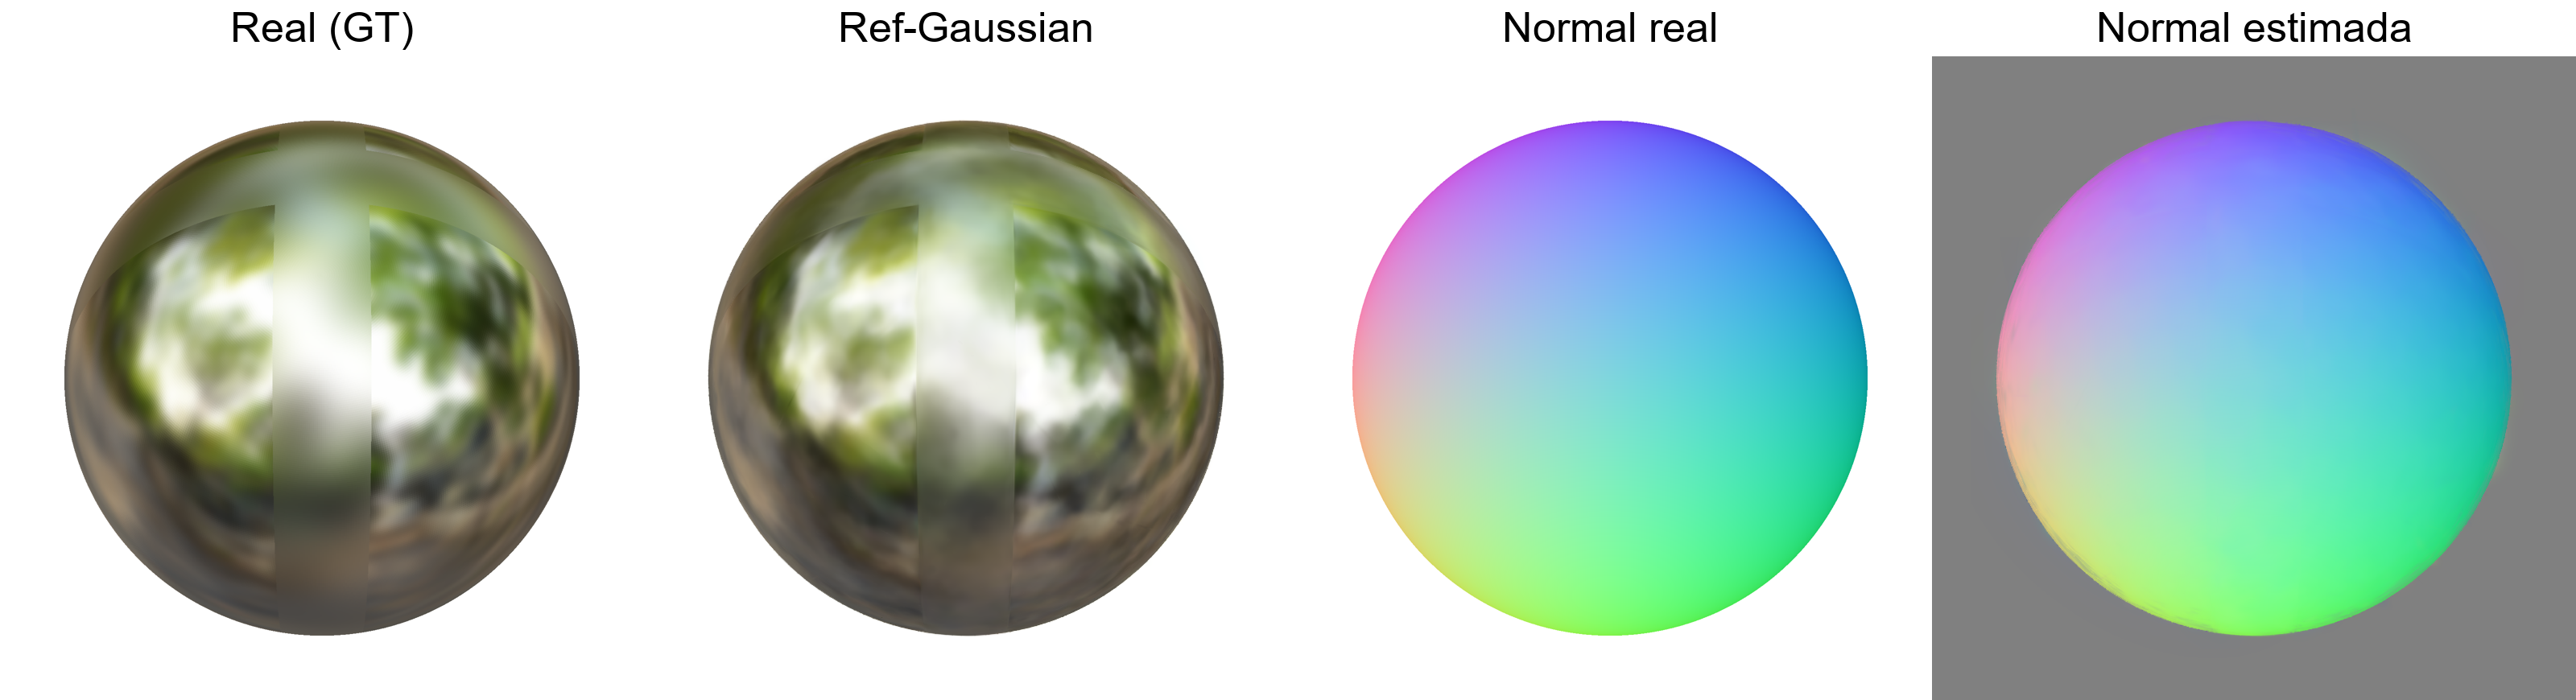
\includegraphics[width=0.8\textwidth]{figs/ball_qualitativo.png}\\[2pt]
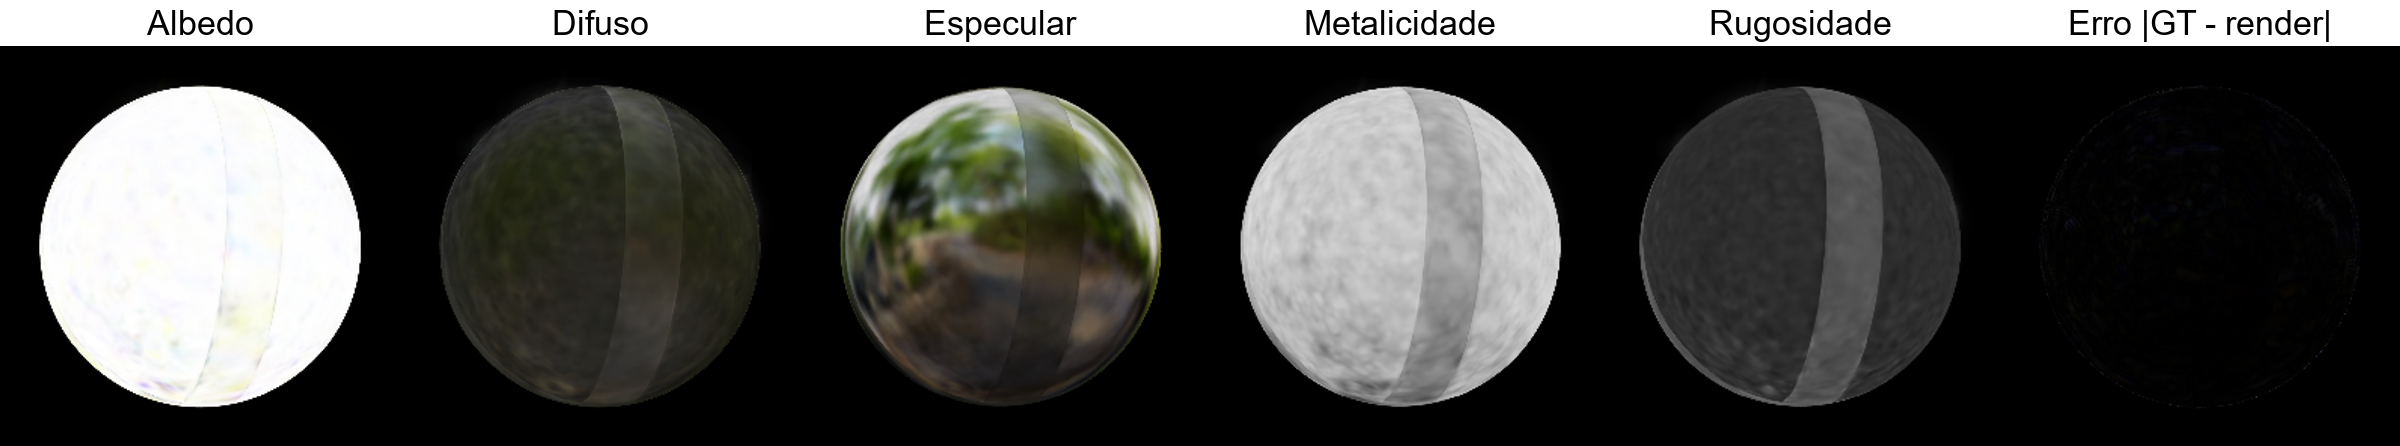
\includegraphics[width=\textwidth]{figs/ball_decomposicao.png}
\caption{Cena \textit{ball}, convexa e sem inter-reflexões. Acima: imagem real, renderização, normal real e normal estimada (vista de teste 0). Abaixo: mapas intermediários da renderização diferida (vista de treino). A faixa mais rugosa da esfera aparece clara na rugosidade e mais escura na metalicidade.}
\label{fig:ball}
\end{figure*}

\textbf{Análise por vista.} A média de 27,51~dB esconde uma variação grande entre vistas (Fig.~\ref{fig:vistas}). O PSNR por vista tem desvio-padrão de 2,58~dB e vai de 18,36 a 33,50~dB; 32 das 200 vistas ficam abaixo de 25~dB. A curva ao longo das vistas, que percorrem uma trajetória em torno do objeto, mostra que as quedas se concentram em faixas contíguas de ângulos, e não em vistas isoladas. Isso indica que o erro depende da geometria de observação, ou seja, de quais regiões do ambiente cada superfície reflete naquela vista. A Fig.~\ref{fig:extremos} compara os extremos. Na melhor vista, a face frontal reflete um ambiente suave e o erro fica restrito às bordas. Na pior, a lateral espelhada da torradeira, que na imagem real reflete uma região escura próxima, é renderizada com um reflexo claro e mal posicionado, e o erro se concentra nessa área. Esse tipo de falha é compatível com uma estimativa incorreta de visibilidade ou de luz indireta: se o raio refletido não é marcado como ocluído, o modelo usa a iluminação distante do mapa de ambiente onde deveria haver luz próxima e escura. A confirmação dessa hipótese, por exemplo inspecionando o mapa de visibilidade nessa vista, é um dos primeiros experimentos previstos para P1 e P2.

\begin{figure*}[t]
\centering
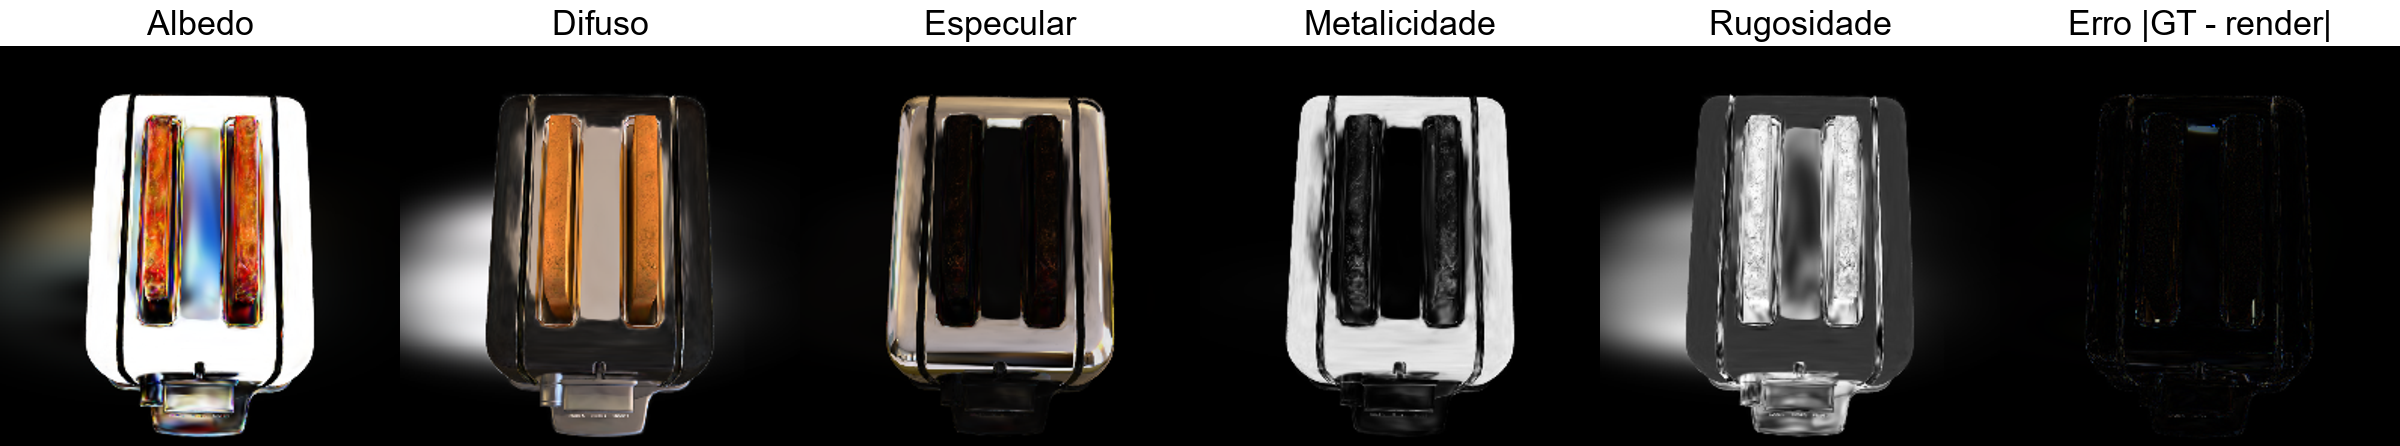
\includegraphics[width=\textwidth]{figs/toaster_decomposicao.png}
\caption{Mapas intermediários da renderização diferida na cena \textit{toaster} (iteração 50.000, vista de treino): albedo, componentes difusa e especular, metalicidade, rugosidade e erro absoluto em relação à imagem real.}
\label{fig:decomp}
\end{figure*}

\begin{figure}[t]
\centering
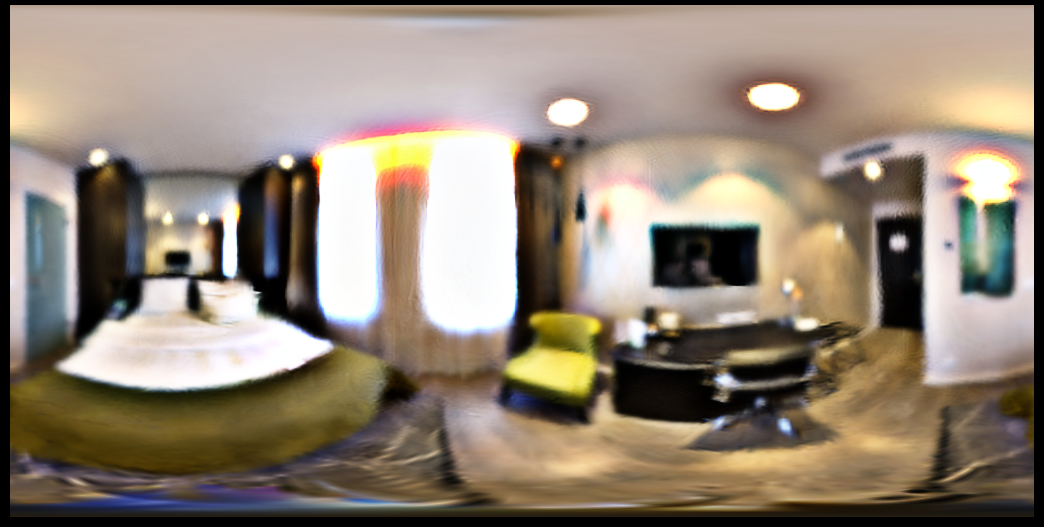
\includegraphics[width=\columnwidth]{figs/toaster_envmap.png}
\caption{Mapa de ambiente aprendido na cena \textit{toaster} (projeção equirretangular), reconstruído apenas a partir dos reflexos observados no objeto.}
\label{fig:envmap}
\end{figure}

\textbf{Decomposição de material e iluminação.} A renderização diferida permite inspecionar separadamente os fatores que o modelo aprendeu (Fig.~\ref{fig:decomp}). A separação física é em grande parte coerente: o corpo da torradeira recebe metalicidade alta e rugosidade baixa, e as fatias de pão recebem metalicidade baixa e rugosidade alta, de modo que a componente especular fica concentrada no metal e a difusa no pão. A decomposição, porém, não é limpa. O albedo da região entre as fatias apresenta cores espúrias, azuladas e iridescentes, que não existem no objeto; a rugosidade varia em manchas sobre o metal, que deveria ser uniforme; e todos os mapas mostram um halo de Gaussianas de baixa opacidade fora do objeto, à esquerda. Os autores atribuem justamente à aproximação de visibilidade parte do ruído na estimativa de materiais, e esta observação dá uma forma qualitativa e mensurável a essa limitação: as métricas de imagem quase não são afetadas, já que o erro final é baixo, mas os materiais recuperados são menos confiáveis do que a renderização sugere. Para aplicações que dependem dos materiais, como reiluminação e inserção de objetos em realidade aumentada, esse é o aspecto mais relevante a melhorar. A Fig.~\ref{fig:envmap} mostra o mapa de ambiente aprendido. O modelo reconstrói, apenas a partir dos reflexos, um ambiente interno reconhecível, com janelas, luminárias, uma cama e uma poltrona, embora borrado e com distorções nas regiões pouco vistas pelos reflexos, como a parte inferior do mapa.

\textbf{Cena convexa versus côncava.} A cena \textit{ball} (Fig.~\ref{fig:ball}) funciona como um controle natural para a análise da \textit{toaster}. Por ser uma esfera, uma superfície convexa, nenhum ponto reflete outra parte do próprio objeto: a visibilidade ao longo de qualquer direção de reflexão é sempre 1, e a aproximação da Eq.~\eqref{eq:vis} é exata. Os sintomas observados na \textit{toaster} praticamente desaparecem. O PSNR por vista tem desvio-padrão de 1,90~dB, contra 2,58~dB na \textit{toaster}, e o mínimo é de 31,66~dB, sem nenhuma vista abaixo de 25~dB. As normais estimadas coincidem visualmente com as reais, e a decomposição recupera a estrutura do material: a faixa mais rugosa que atravessa a esfera aparece com rugosidade maior e metalicidade menor, e a componente especular reflete o ambiente com nitidez. O ruído não some totalmente, pois a metalicidade ainda apresenta manchas sobre uma superfície que deveria ser uniforme, mas é bem menor que o da \textit{toaster}. A comparação é limitada a duas cenas e as diferenças entre elas não se devem só à convexidade (os materiais e ambientes também diferem), mas é consistente com a hipótese de que a modelagem de visibilidade é o principal fator nos casos difíceis.

\textbf{Síntese.} Os resultados desta etapa indicam que (i) o baseline é reproduzível em hardware de consumo, com métricas próximas às do artigo nas duas cenas concluídas; (ii) a qualidade média esconde falhas localizadas, ligadas a vistas em que as superfícies refletem regiões próximas, e essas falhas praticamente não ocorrem na cena convexa; e (iii) os materiais recuperados são ruidosos mesmo quando a imagem renderizada é fiel, em especial na cena côncava. Os pontos (ii) e (iii) são precisamente os efeitos esperados da aproximação de visibilidade do baseline, o que reforça a escolha de P1 e P2 como linhas de investigação.

\textbf{Próximos passos.} (i) Concluir as quatro cenas restantes do Shiny Blender e completar a Tabela~\ref{tab:replicacao}; (ii) estender a replicação ao Glossy Synthetic e ao Shiny Blender Real; (iii) instrumentar o código para medir separadamente o custo da extração de malha e do ray tracing; (iv) exportar os mapas de visibilidade e de luz indireta nas vistas de maior erro, para testar a hipótese levantada na análise por vista; e (v) implementar uma primeira versão de P1 com $K$ pequeno e compará-la ao baseline.

% =====================================================================
\section{Conclusão}

Este relatório apresentou o método Ref-Gaussian, adotado como baseline da dissertação, e discutiu duas de suas limitações: a visibilidade testada em uma única direção e a dependência de uma malha extraída periodicamente. Para cada uma foi proposta uma linha de investigação. O baseline foi portado para Windows e executado em uma GPU de notebook, e a replicação reproduziu os resultados do artigo nas duas cenas concluídas. O PSNR ficou 0,54~dB abaixo na \textit{toaster} e 0,94~dB abaixo na \textit{ball}, com SSIM e LPIPS iguais ou melhores que os reportados. A análise por vista, a decomposição de material e o contraste entre uma cena côncava e uma convexa mostraram dois sintomas que serão usados como referência para avaliar as propostas: erros concentrados em vistas nas quais as superfícies refletem regiões próximas e materiais ruidosos sob uma renderização fiel.

\begin{thebibliography}{00}
\bibitem{kerbl2023} B. Kerbl, G. Kopanas, T. Leimkühler, and G. Drettakis, ``3D Gaussian splatting for real-time radiance field rendering,'' \textit{ACM Trans. Graph.}, vol. 42, no. 4, 2023.
\bibitem{huang2024_2dgs} B. Huang, Z. Yu, A. Chen, A. Geiger, and S. Gao, ``2D Gaussian splatting for geometrically accurate radiance fields,'' in \textit{Proc. ACM SIGGRAPH}, 2024.
\bibitem{yao2025refgaussian} Y. Yao, Z. Zeng, C. Gu, X. Zhu, and L. Zhang, ``Reflective Gaussian splatting,'' in \textit{Proc. Int. Conf. Learn. Represent. (ICLR)}, 2025.
\bibitem{jiang2024gaussianshader} Y. Jiang, J. Tu, Y. Liu, X. Gao, X. Long, W. Wang, and Y. Ma, ``GaussianShader: 3D Gaussian splatting with shading functions for reflective surfaces,'' in \textit{Proc. IEEE/CVF Conf. Comput. Vis. Pattern Recognit. (CVPR)}, 2024.
\bibitem{ye2024dr} K. Ye, Q. Hou, and K. Zhou, ``3D Gaussian splatting with deferred reflection,'' in \textit{Proc. ACM SIGGRAPH}, 2024.
\bibitem{verbin2022refnerf} D. Verbin, P. Hedman, B. Mildenhall, T. Zickler, J. T. Barron, and P. P. Srinivasan, ``Ref-NeRF: Structured view-dependent appearance for neural radiance fields,'' in \textit{Proc. IEEE/CVF Conf. Comput. Vis. Pattern Recognit. (CVPR)}, 2022.
\bibitem{liu2023nero} Y. Liu, P. Wang, C. Lin, X. Long, J. Wang, L. Liu, T. Komura, and W. Wang, ``NeRO: Neural geometry and BRDF reconstruction of reflective objects from multiview images,'' \textit{ACM Trans. Graph.}, vol. 42, no. 4, 2023.
\bibitem{karis2013} B. Karis, ``Real shading in Unreal Engine 4,'' in \textit{SIGGRAPH Course: Physically Based Shading in Theory and Practice}, 2013.
\bibitem{moenne2024_3dgrt} N. Moenne-Loccoz, A. Mirzaei, O. Perel, R. de Lutio, J. M. Esturo, G. State, S. Fidler, N. Sharp, and Z. Gojcic, ``3D Gaussian ray tracing: Fast tracing of particle scenes,'' \textit{ACM Trans. Graph.}, vol. 43, no. 6, 2024.
\end{thebibliography}

\end{document}
